\subsection{Creating the Level Set}

Before we create the level set $\phi$ that represent the surface of our water simulation, we need to mark the cells that we consider fluid. The easiest approach is to go from particle position $\vec{x}_p$ to grid coordinates $(i,j)$ and tag that cell as fluid.

\begin{algorithm}
\caption{Marking cells as fluid}
\begin{algorithmic}
\STATE marker = empty grid (all values 0)
\FOR{all particles $p$}
\STATE i,j = int(p.x / $\Delta x$)
\STATE marker(i,j) = 1
\ENDFOR
\end{algorithmic}
\label{markalgorithm}
\end{algorithm}

In Algorithm \ref{markalgorithm}, a cell will most likely contain several particles at once which means that we will write the value $1$ to that cell multiple times. Although unnecessary, this is a very fast operation compared to all the other step in the level set creation and the overhead should not be noticable. Figure \ref{markerexample} shows and example of the marker grid after we run Algorithm \ref{markalgorithm} on an input of particles. Notice that cells with only one particle is still counted as a fluid cell.

\begin{figure}[ht!]
\centering
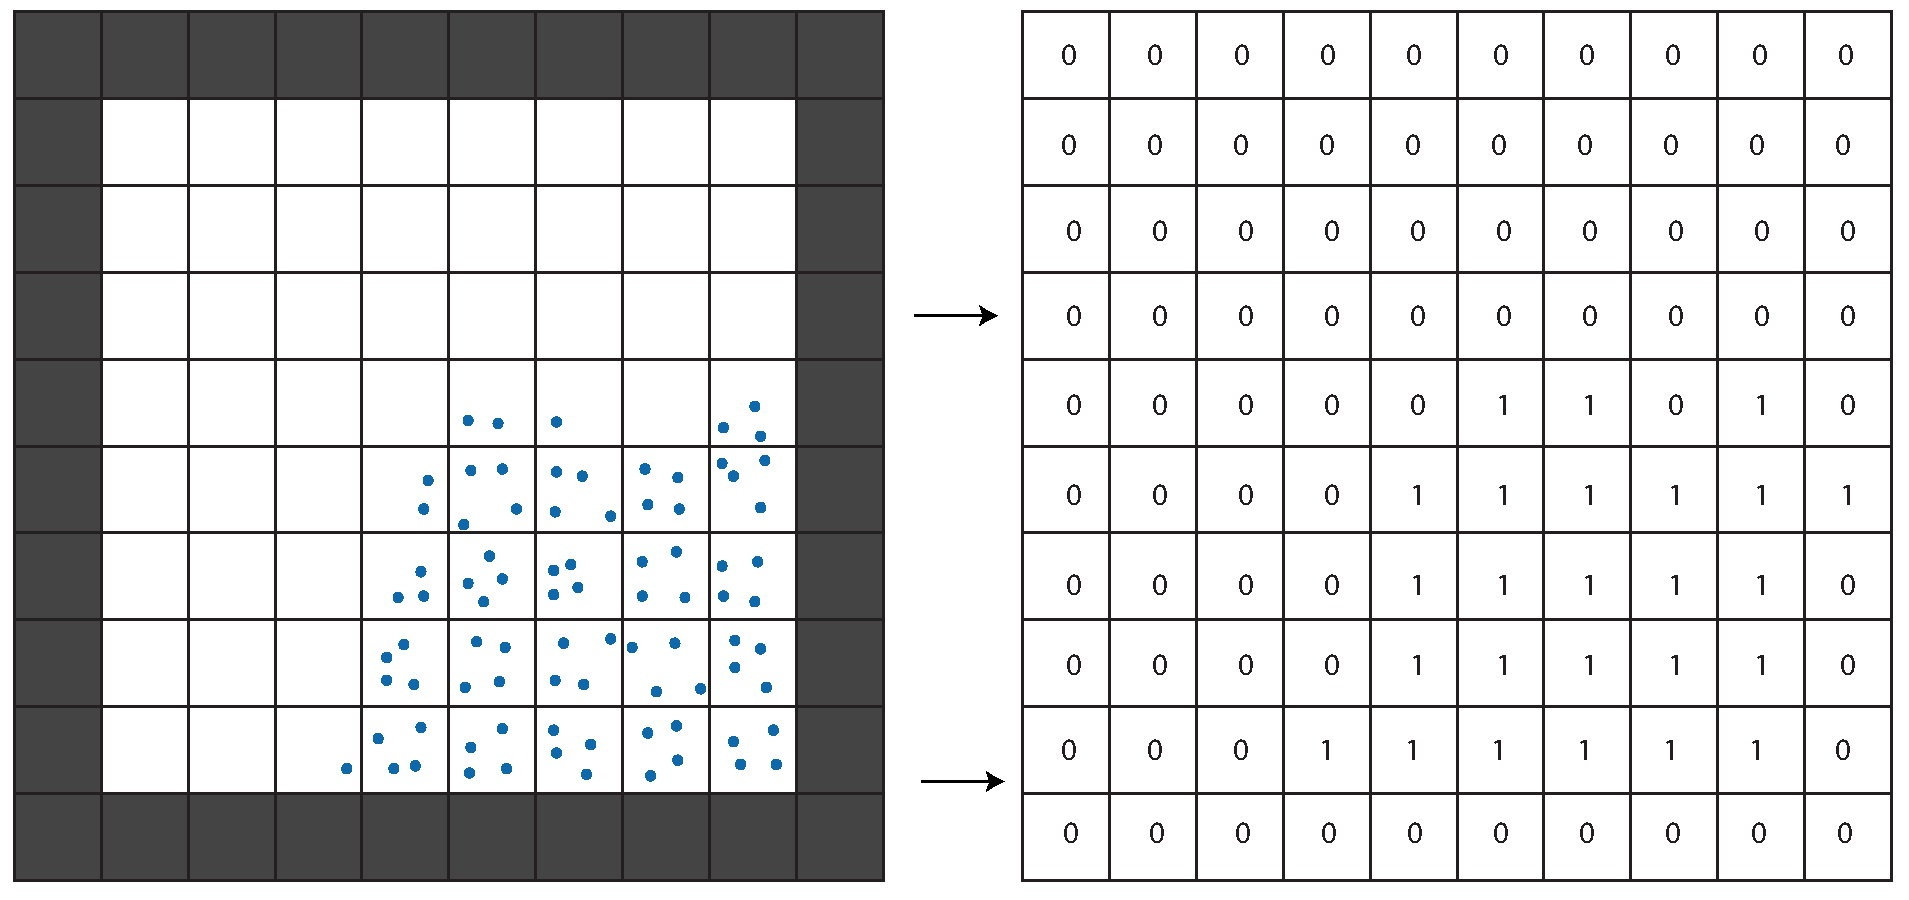
\includegraphics[width=130mm]{img/mark.pdf}
\caption{Cells with particles inside them as are marked as fluid cells.}
\label{markerexample}
\end{figure}

Then next step in the algorithm is to initialize the level set. This step will not create a valid level set that satisfies Equation \ref{eikonaleqfirst}. To start with, we are just going to set $\phi_{i,j}$ to $-\frac{\Delta x}{2}$ as if the surface could be at the edge of the cell. To cells not marked as fluid we will set the value to $D \cdot \Delta x$ where it is important that $D >> \Delta X$. Typically the initalizing step was run with $D = 1000$.

\begin{algorithm}
\caption{Initalizing the Level Set}
\begin{algorithmic}
\STATE marker = ... (marker grid from Algorithm \ref{markalgorithm})
\STATE inside = -0.5 * $\Delta x$
\STATE outside = D * $\Delta x$
\FOR{$i=0$ to $N_x$}
\FOR{$j=0$ to $N_y$}
\IF{marker(i,j) is 1}
\STATE phi(i,j) = inside
\ELSE
\STATE phi(i,j) = outside
\ENDIF
\ENDFOR
\ENDFOR
\end{algorithmic}
\label{particlestogridalgorithm2}
\end{algorithm}

After this initializing step, the level set is far from continous. To make it continuous and satisfy $|\nabla \phi| = 1$, we are going to perform an iterate sollver of the Eikonal equation. This step is sometimes called the reinitializing step in level set literature.
